\section{Area distribution}

The modular distribution of the structure is automated by an algorithm from which the user can interact directly by telling the software the general dimensions (width, height and length), separation between joists, modular subdivisions and load distribution. Moreover, it was designed to be flexible enough to adapt for complex geometries. For example, lets suppose that a client has a warehouse of six by six meters of area and wants a structure with three meters of height which has to support $700 \left[kg/ m^2 \right]$, but the building has a column in the middle of it with square dimensions of $0.5 [m]$. A possible solution for this problem can be appreciated on Figure \ref{area}.

\vspace{-0.7cm}

\begin{figure}[h!]
\centering
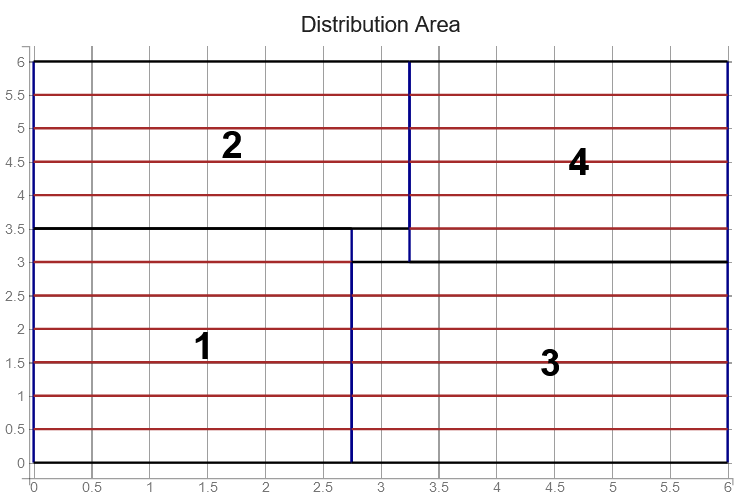
\includegraphics[width=0.9\textwidth]{Images/General/area2.PNG}
\caption{Area distribution of study.}
\label{area}
\end{figure}

\vspace{-0.7cm}

As seen on Figure \ref{area2}, an algorithm of \textit{Object Oriented Programming} (OOP) has been implemented to the automatic distribution of the area, using RAM memory\footnote{Off course, this can be changed to be stored on the HDD memory rather than RAM memory, if needed.} to store the dimensions of each module, in this case: 1, 2, 3 and 4. An object of the module was created which uses $x$ and $y$ position to know its position in the space, $L$ and $W$ parameters referring to \textit{length} and \textit{width}, respectively, and a `Delete' checkbox to erase the module (not used in this example).

\begin{figure}[h!]
\centering
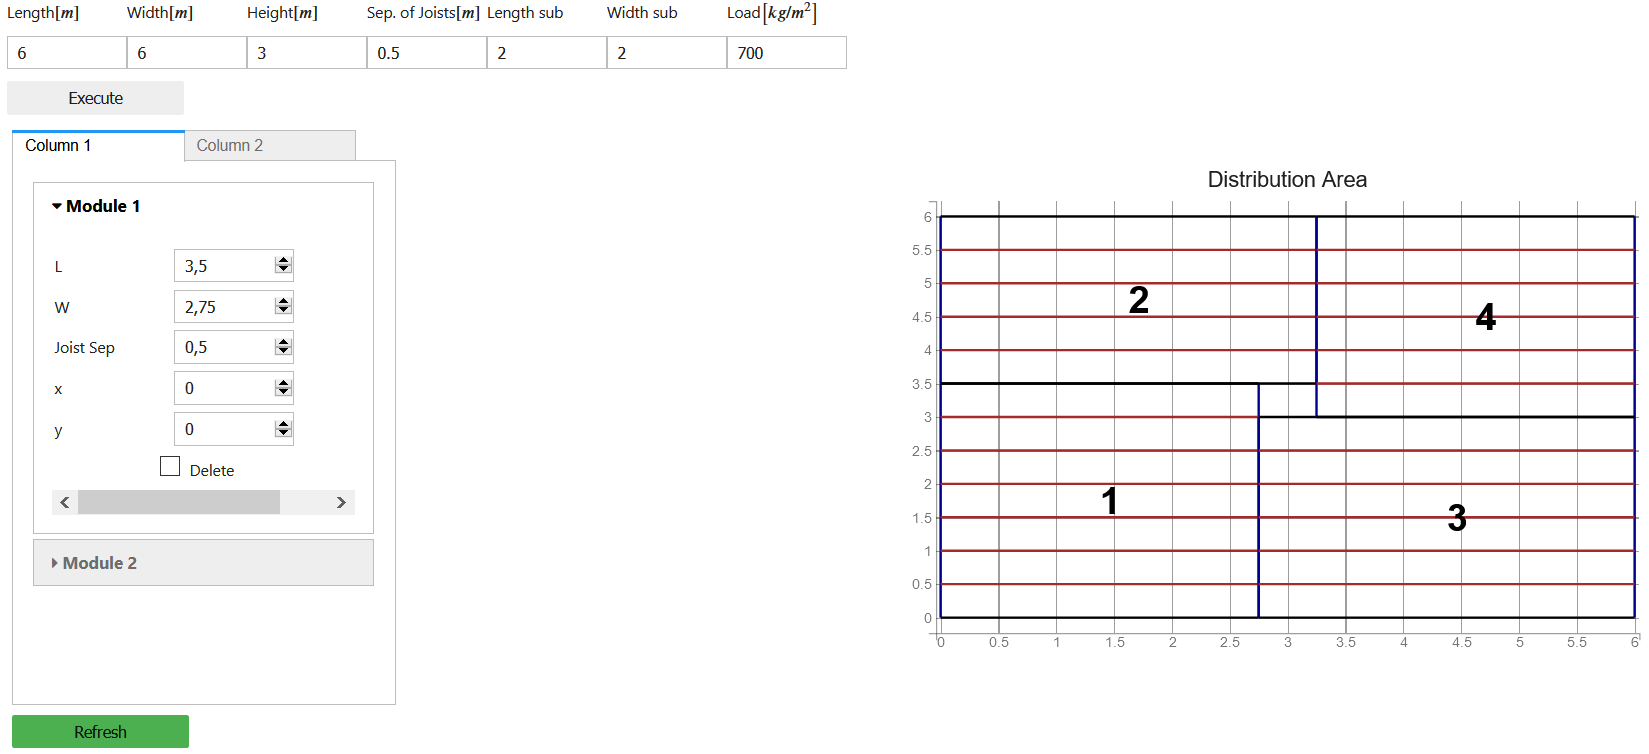
\includegraphics[width=0.88\textwidth]{Images/General/area.PNG}
\caption{User interface of the area distribution.}
\label{area2}
\end{figure}